The heavy photon, also known as the A$^{\prime}$, is a theoretically motivated massive gauge boson that is associated with a predicted U(1) hidden symmetry, favorable to Beyond Standard Model theories. According to theory~\cite{holdom_two_1986}, a heavy photon kinetically mixes with the Standard Model photon through a loop-level effect generating an effective coupling to electric charge. This coupling to electric charge, $\epsilon$, can range from $10^{-12}$ to $10^{-2}$ depending on loop order of the mixing interaction and describes the coupling of the heavy photon to electric charge to be at a scale significantly smaller than that in standard electrodynamic theory. While the coupling strength of the interaction can be naturally generated from the loop interactions, the mass is somewhat less constrained. Theories of the heavy photon as a way to explain cosmological phenomena make them the simplest and possible leading interaction between the Standard Model and the Dark Sector. The Dark Sector encompasses both dark matter and dark energy particles that we cannot interact with other than the observed gravitational effects. If the heavy photon should obtain its mass through the Higgs mechanism, the mass is favored to be in the range of MeV to GeV which is compatible with dark matter theories. In such a scenario, electrons could radiate heavy photons as they do ordinary photons but at a suppressed rate. These heavy photons will have measurable lifetimes before decaying to charged particle pairs. It is natural to describe the heavy photon parameter space in terms of its coupling, $\epsilon^2$, and mass, $m_{A'}$. \\
\indent The Heavy Photon Search (HPS) experiment searches for heavy photons in the range of 20 to 1000~MeV/c$^2$ range with prompt or displaced vertices with respect to the target interaction. HPS is sensitive to heavy photons radiated from an electron beam incident on a heavy target by measuring the momentum and vertex position of $e+e-$ pairs produced from decay. By reconstructing the invariant mass and the vertex position of the pairs, HPS can look for a small bump on a large background using a bump hunt for prompt decays. Uniquely, HPS is also able to look for heavy photons with smaller couplings (and longer lifetimes) characterized by displaced vertices by searching for a small signal on low background downstream of the target. The mass and coupling region that HPS seeks to explore is shown in gold in Figure~\ref{Figure:projReach} along with the existing limits from other experiments. 

\begin{figure}[H]
  \centering
      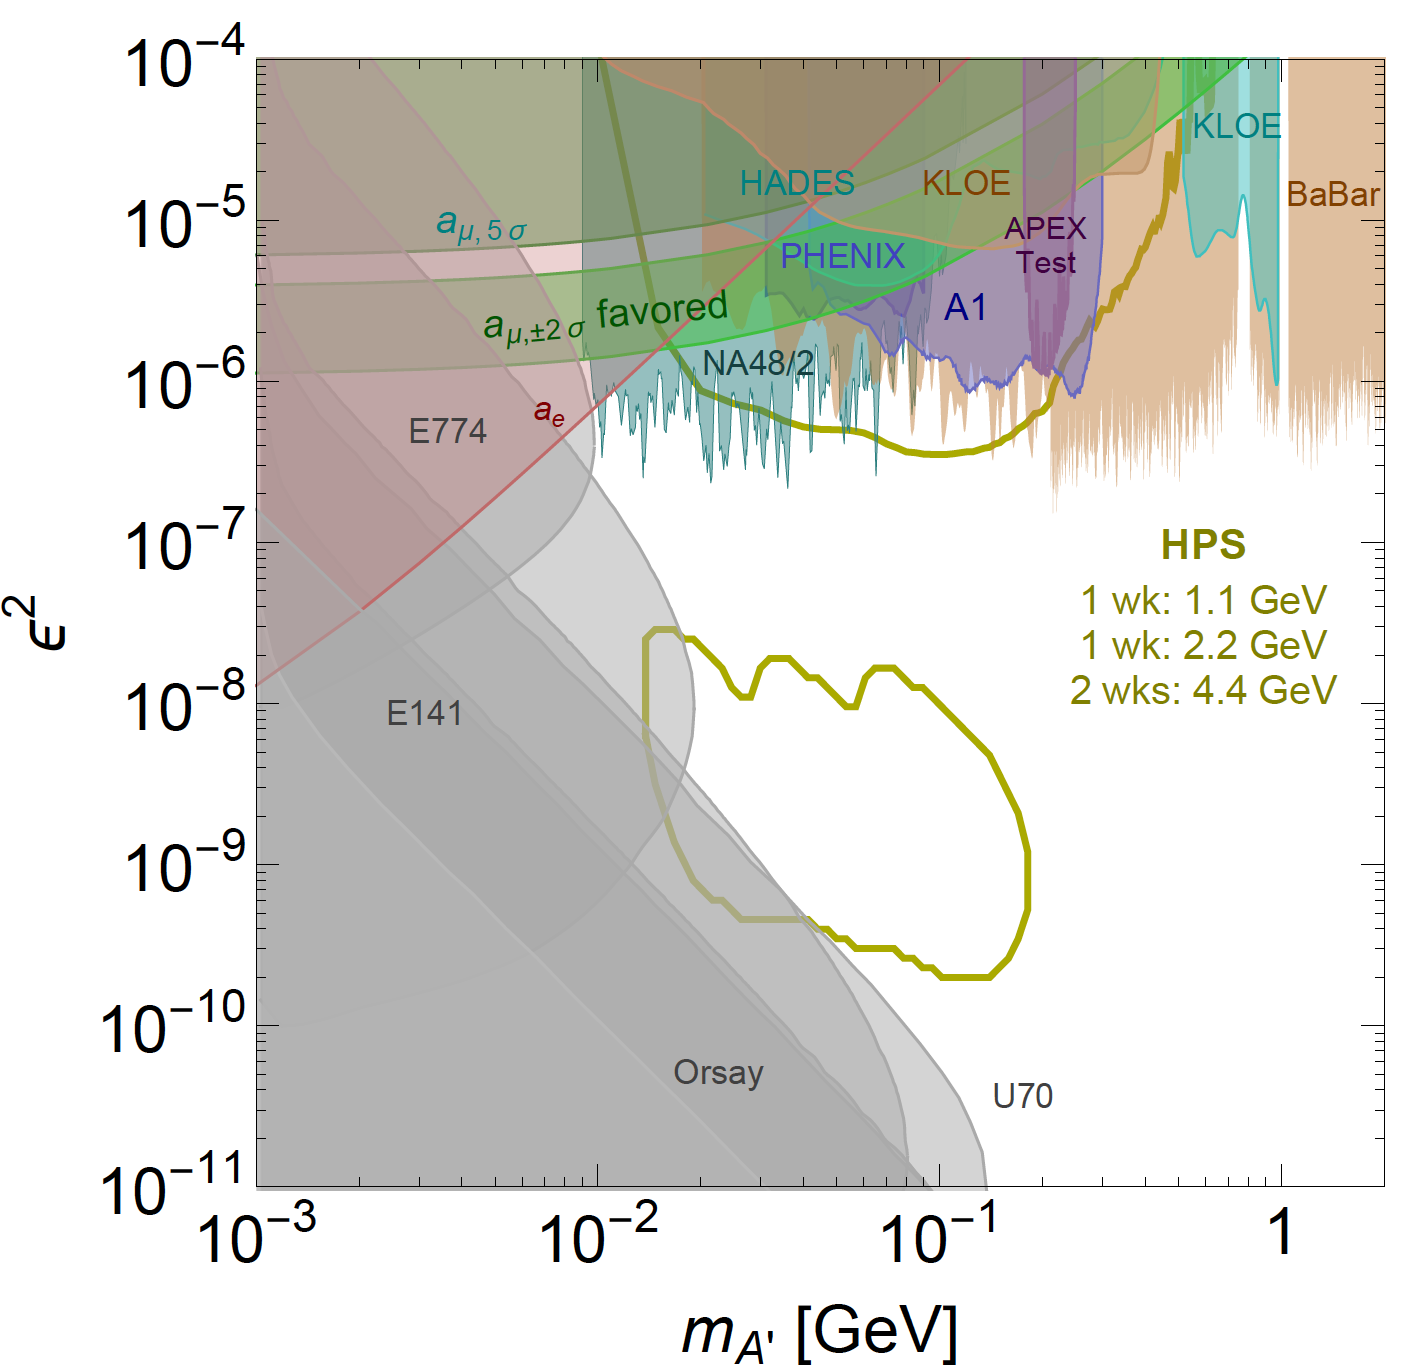
\includegraphics[width=0.6\textwidth]{pics/intro/projectedReach.png}
  \caption[Projected reach for the HPS experiment]{The existing 90$\%$ confidence limits from other experiments looking for heavy photons in the relevant mass-coupling region is shown. The gold contours indicate the projected reach from the full running of the HPS experiment according to the proposal~\cite{collaboration_heavy_2013}. The green bands labeled as $a_\mu$ indicate the favored parameter space for a visibly decaying heavy photon to explain the discrepancy between the calculated and measured muon anomalous magnetic moment The experiments along the top of the plot with large coupling look for heavy photons that decay promptly at the target. The limits shown in grey along the left side of the plot with decreasing values of coupling look for heavy photons with displaced vertices in beam dump experiments.}
  \label{Figure:projReach}
\end{figure}

The HPS experiment took place in Hall B at the Jefferson Laboratory National Accelerator Facility. The Continuous Electron Beam Accelerator Facility (CEBAF) at Jefferson Lab produces an electron beam that collides with the HPS target material in Hall B. The HPS detector measures the particles from this interaction and searches for the heavy photon signal. The HPS detector is consists of a Silicon Vertex Tracker (SVT) and an Electromagnetic Calorimeter (ECal). The SVT is composed of six layers of silicon strips and is housed in a magnetic field. The SVT measures particle tracks and reconstructs the vertex position of the particle pair. The ECal triggers event readout in addition to measuring particle energy and pair coincidence timing. \\
\indent The ECal was commissioned during a short commissioning run in December 2014. The full experiment ran in the spring of 2015 as the official Engineering Run. This run took 2.3~days of good data at approximately 50~nA with a beam energy of 1.056~GeV. HPS obtained a total of 1529~nb$^{-1}$ of good data. Due to the commissioning of the SVT during the Engineering Run, the SVT was not moved into its nominal position at $\pm0.5$~mm from the beam until later in the running, and data was taken with the SVT slightly open at $\pm1.5$~mm from the beam.  Further experimental running took place during the spring 2016 Physics Run with a 200~nA electron beam at 2.3~GeV collecting a total of 5.7~days of data.  Future running at higher electron beam energy is planned for 2018 and beyond.\\
\indent This dissertation searches for heavy photons with a displaced vertex using data from the Engineering Run with the SVT at $\pm0.5$~mm and $\pm1.5$~mm from the beam. I will give an overview of the experiment as a whole with detail to the areas of which I was most involved with. Significant effort was made to study the vertex analysis in the context of a blinded analysis by using 10$\%$ of the data. In order to better understand and analyze the backgrounds in the vertex search, I conducted a detailed study of the backgrounds using the statistics of the fully unblinded dataset. In addition to the full vertex analysis, I contributed significantly to the assembly, characterization and commissioning of the Ecal for all experimental running. I wrote the clustering algorithm based on that used by the CLAS experiment Inner Calorimeter (IC) and improved simulations of the ECal detector. 
